\subsection{Ecommerce websites vs news websites}
In our research, a crucial element was the comparison of two types of websites. This comparison enabled us, firstly, to hypothesize about the potential uses of cross-device tracking and, secondly, to understand when user data is more susceptible to being shared with third parties. We compared online shopping sites and news websites. This choice of categories was driven by the common use of cross-device tracking, which is typically needed either for advertising purposes, beneficial to sales-focused companies, or for targeting specific audiences, a tactic often employed by political entities. At the beginning of our study, we assumed that cross-device tracking would be more prevalent in online stores. However, the data we gathered did not confirm our assumptions. Instead, we were able to draw interesting conclusions about how these two types of sites collect and use sensitive user data, and what potential risks there might be for the users.

\subsubsection{Comparing Third-party requests}
\noindent 
\begin{minipage}{0.4\textwidth} 
    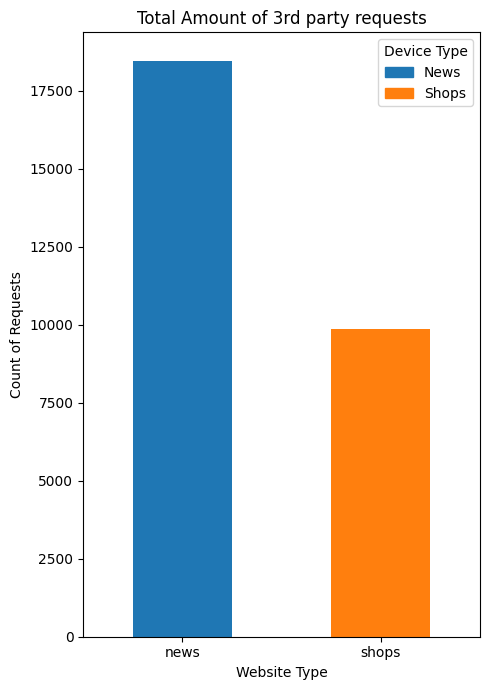
\includegraphics[width=\linewidth]{./assets/comparison1.png} 
\end{minipage}%
\hfill 
\begin{minipage}{0.5\textwidth} 
    One of the key aspects for comparison are third-party requests, as they are a primary indicator that sensitive data might be shared with third parties to create a more accurate user profile. We decided to find out which type of website makes more third-party requests. The chart demonstrates that in our dataset, news websites sent almost twice as many requests as online stores. This could be due to the fact that news websites almost always have more advertising, trackers for analytics, or social media widgets, which require reaching out to third-party servers. This makes such sites an ideal environment for cross-device tracking, and thus for collecting the maximum amount of user data.
\end{minipage}

\subsubsection{Comparing cookies set}
Cookies are a very important step in linking a user's activity on one device with their activity on another. Cookies also store information about the pages viewed, the time of site visits, and even the user's interaction scenario with the site, which are crucial for cross-device tracking.

\vspace{0.8cm}
\noindent 
\begin{minipage}{0.6\textwidth} 
    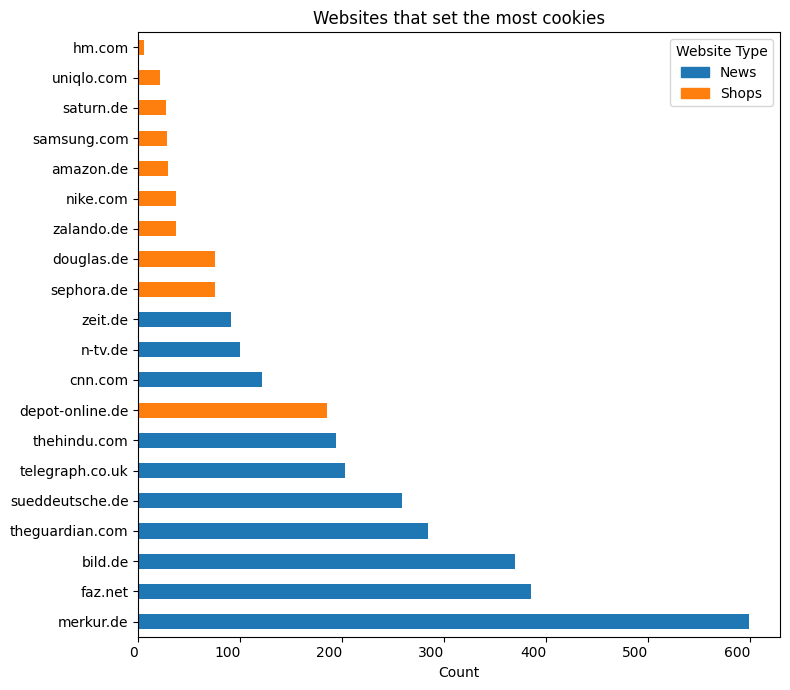
\includegraphics[width=\linewidth]{./assets/comparison21.png}
\end{minipage}
\hfill 
\begin{minipage}{0.35\textwidth}
    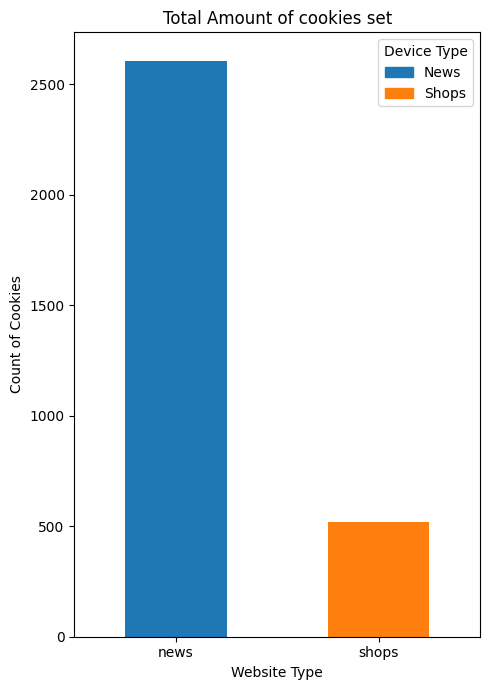
\includegraphics[width=\linewidth]{./assets/comparison2.png}
\end{minipage}


\subsubsection{Shared email addresses}
\noindent 
\begin{minipage}{0.4\textwidth} 
    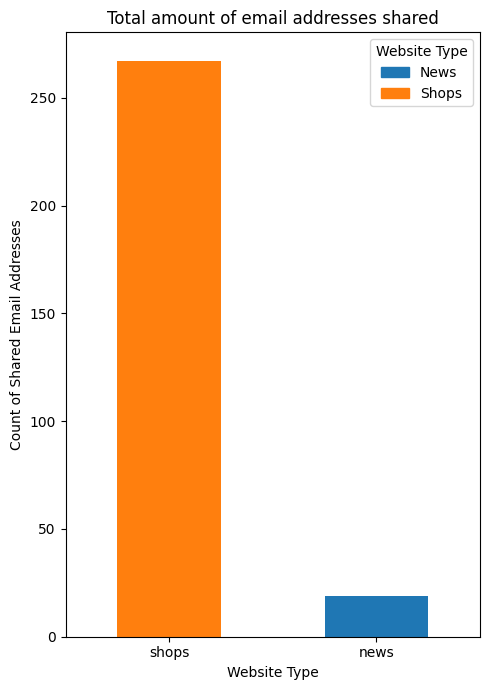
\includegraphics[width=\linewidth]{./assets/comparison3.png} 
\end{minipage}
\hfill 
\begin{minipage}{0.5\textwidth} 
    One of the most interesting findings of our research is the fact that online stores distributed email addresses more than ten times as often as news websites. The email address is a key identifier for linking a user's various devices. Therefore, it can be concluded that online stores also use cross-device tracking to create a unified customer profile, but apparently employ methods different from those used by news platforms. As noted earlier, the company Sephora initiated a significant portion of the email address transfers, raising concerns about the privacy of data used by this company. In any case, such research results could be due to the fact that sales-oriented websites are more interested in retaining customers by offering personalized discounts and deals via email, while for news sites, individual user interaction is not as crucial as content and advertising targeting.
\end{minipage}
\vspace{0.8cm}

\subsection{Mobile vs desktop}
We compared mobile and desktop devices in terms of the total amounts of each analysis category and noticed that data collection varied across different devices.

\vspace{0.8cm}
\noindent 
\begin{minipage}{0.35\textwidth} 
    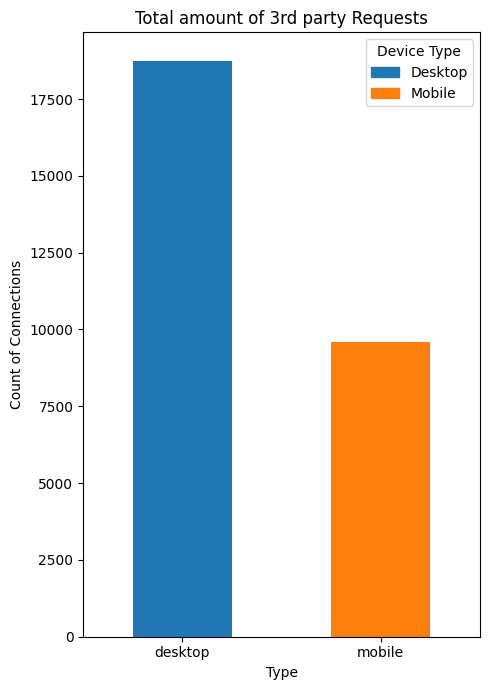
\includegraphics[width=\linewidth]{./assets/comparison5.png} 
\end{minipage}
\hfill 
\begin{minipage}{0.6\textwidth} 
    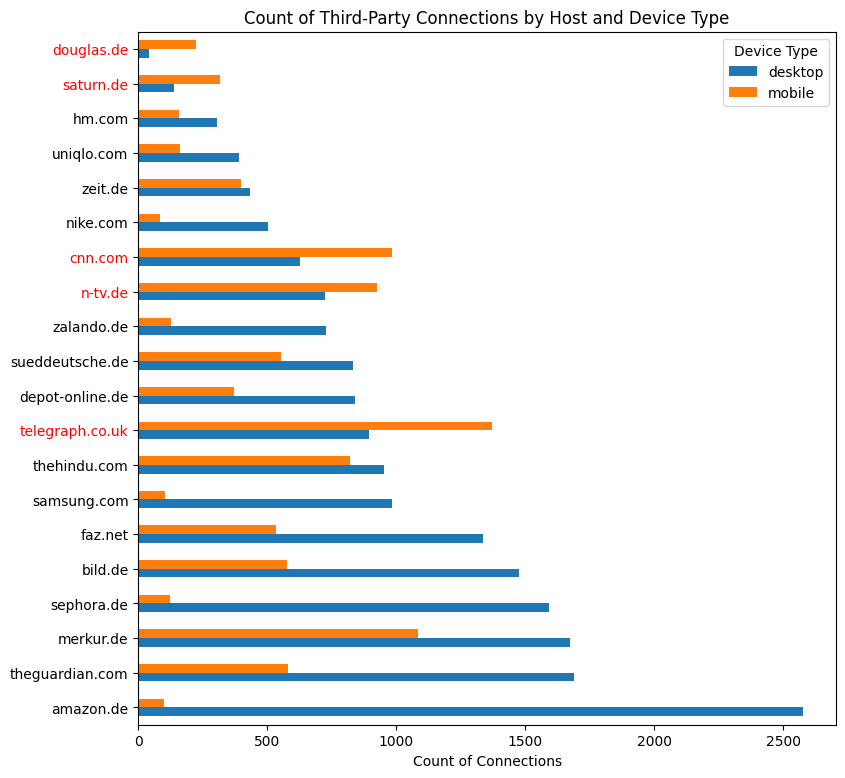
\includegraphics[width=\linewidth]{./assets/comparison51.png} 
\end{minipage}
\vspace{0.8cm}

For example, desktop devices showed more involvement from third parties. 15 out of 20 sites used more third-party connections on desktop devices than on mobile devices. The reason might be that desktop versions of websites are usually more extensive, incorporating more advertising networks, which initiates more communication with external servers. Additionally, users are likely to prefer desktop devices for more involved interactions with a website (such as making purchases, payments, registering on a site, or generally using the site for an extended period), so it is very beneficial for companies to implement cross-device tracking in the desktop versions of their websites.

\vspace{0.8cm}
\noindent 
\begin{minipage}{0.45\textwidth} 
    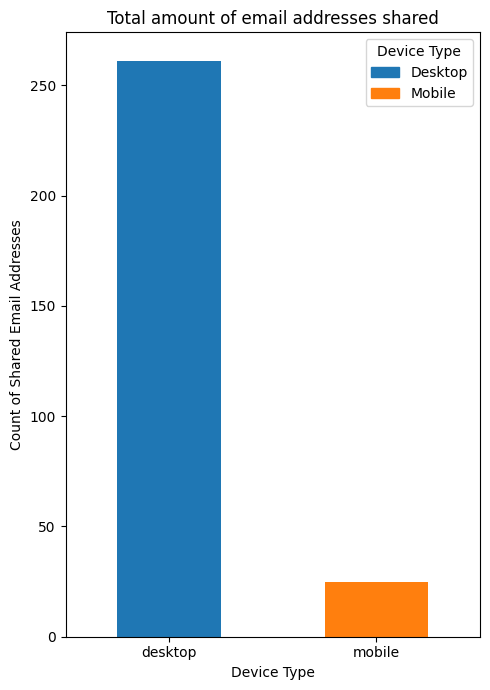
\includegraphics[width=\linewidth]{./assets/comparison4.png} 
\end{minipage}
\hfill 
\begin{minipage}{0.45\textwidth} 
    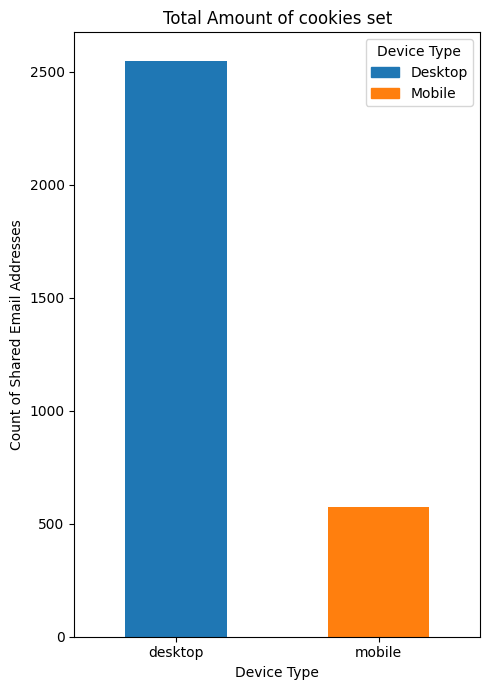
\includegraphics[width=\linewidth]{./assets/comparison6.png} 
\end{minipage}
\vspace{0.8cm}

A similar trend is observed in the setting of cookie files and the transfer of email addresses. It appears that website owners prefer to use traditional PCs as the primary target for long-term user data tracking, while mobile devices serve as an additional source after creating a unified user profile through cross-device tracking. This strategy uses the strengths of each device type. Desktops are used for detailed data collection and in-depth user interactions, while mobile devices supplement this information, providing insights into on-the-go behaviors and preferences. This combination ensures a more complete picture of the user's online interaction.